\chapter{História da Criptografia Quântica}

A história da criptografia quântica pode ser rastreada até a década de 1980, quando os pesquisadores começaram a explorar o potencial de usar a mecânica quântica para codificar e transmitir informações de maneira segura. Uma das primeiras ideias nesse campo foi o conceito de distribuição de chaves quânticas (QKD), que permite a troca segura de chaves criptográficas em um canal quântico.

O primeiro protocolo QKD foi proposto por Charles Bennett e Gilles Brassard em 1984 e agora é conhecido como protocolo BB84. Este protocolo é baseado nos princípios da mecânica quântica e usa fotões para codificar e transmitir informações.

\begin{figure}[!hbt]
  \centering
  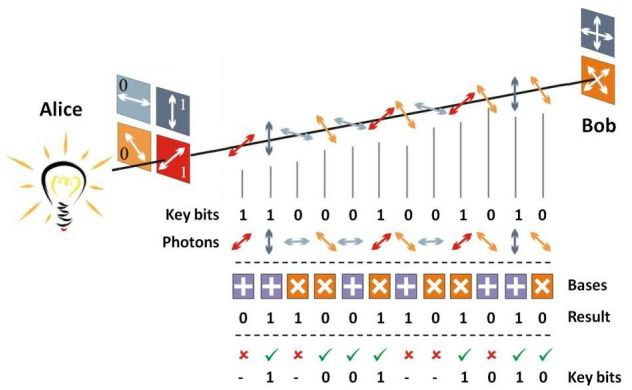
\includegraphics[width=\textwidth]{images/cool-bb84.jpg}
  \caption{Figura ilustrativa do protocolo BB84.}
  \label{fig:cool-bb84}
\end{figure}
\FloatBarrier

Ao longo dos anos, muitos outros protocolos QKD foram propostos e estudados, incluindo o protocolo B92, o protocolo E91 e o protocolo SARG04. Esses protocolos demonstraram oferecer vantagens significativas em relação à criptografia clássica, incluindo segurança incondicional e a capacidade de detectar e impedir espionagem.

Na década de 1990, várias demonstrações experimentais de QKD foram realizadas, mostrando que os princípios da criptografia quântica poderiam ser implementados na prática. Nos anos 2000, vários sistemas QKD comerciais foram desenvolvidos e implantados, marcando o início de uma nova era na comunicação segura.

Hoje, a criptografia quântica é um campo em rápido desenvolvimento, com muitos pesquisadores e empresas trabalhando em novos protocolos, tecnologias e aplicações. Apesar dos muitos desafios que permanecem, a promessa da criptografia quântica é clara e é provável que esse campo continue a desempenhar um papel importante no futuro da comunicação segura.

\newpage
